\section{\acs{SNTP} Over The Internet}\label{sec:sntp_over_the_internet}
When using \ac{SNTP} over the Internet, the goal is to get the offset of every device in the network, master and slave, relative to a third-party \ac{NTP}-server.
\ac{NTP} and \ac{SNTP} works by sending timestamped packages from the slave to the \ac{NTP}-server, and back.
This is illustrated in \cref{fig:ntp_packets}

\begin{figure}[htb]
    \centering
    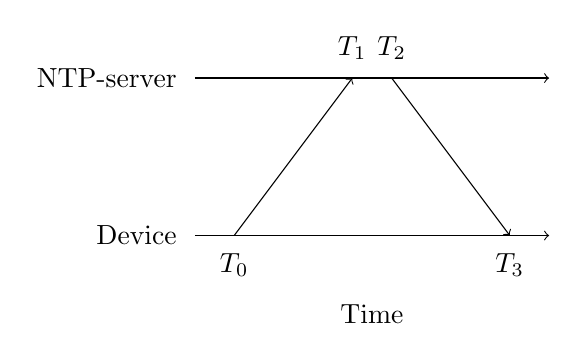
\begin{tikzpicture}[auto]
        \draw[->] (0, 0) -- (4.5, 0);
        \draw[->] (0,-2) -- (4.5,-2);

        \draw[->] (0.5, -2) -- (2, 0);
        \draw[->] (2.5, 0) -- (4.0, -2);

        \draw (2.25, -3) node {Time} node[above=3pt] {$   $};

        \draw (0,  0) node[left=3pt] {NTP-server};
        \draw (0, -2) node[left=3pt] {Device};

        \draw (0.5, -2) node[below=3pt] {$T_0$};
        \draw (4.0, -2) node[below=3pt] {$T_3$};
        \draw (2  ,  0) node[above=3pt] {$T_1$};
        \draw (2.5,  0) node[above=3pt] {$T_2$};
    \end{tikzpicture}
    \caption{The timestamps sent and received during \ac{NTP} synchronization.}\label{fig:ntp_packets}
\end{figure}

Here $T_0$ is the timestamp, on the device, where the request was sent, $T_1$ is the timestamp, on the \ac{NTP}-server, when the request was received.
$T_2$ is the timestamp, on the \ac{NTP}-server, when the response was sent, and $T_3$, is the timestamp, on the device, when the response was received.
Given this, one can calculate the offset, $\theta$, with the equation\ \ref{eq:ntp}.

\begin{equation}\label{eq:ntp}
    \theta = \frac{(t_1 - t_0)+(t_2 - t_3)}{2}
\end{equation}

When using \ac{NTP} one also have to decide on what \ac{NTP}-server to use.
We decided to use \url{0.dk.pool.ntp.org} which is a free to use \ac{NTP}-pool, and its servers are located in Denmark, furthermore we get a low latency to them, which can improve the accuracy of the synchronization.

